% Gemini theme
% https://github.com/anishathalye/gemini
%
% We try to keep this Overleaf template in sync with the canonical source on
% GitHub, but it's recommended that you obtain the template directly from
% GitHub to ensure that you are using the latest version.

\documentclass[final]{beamer}

% ====================
% Packages
% ====================

\usepackage[T1]{fontenc}
\usepackage{lmodern}
\usepackage[size=custom,width=120,height=91,scale=1.2]{beamerposter}
\usetheme{gemini}
\usecolortheme{gemini}
\usepackage{graphicx}
\usepackage{booktabs}
\usepackage{float}
\usepackage{tikz}
%\usepackage[caption=false]{subfig}
%\usepackage{caption}
\usepackage{subcaption}
%\captionsetup{compatibility=false}
\usepackage{pgfplots}
\pgfplotsset{compat=1.14}

% ====================
% Lengths
% ====================

% If you have N columns, choose \sepwidth and \colwidth such that
% (N+1)*\sepwidth + N*\colwidth = \paperwidth
\newlength{\sepwidth}
\newlength{\colwidth}
\setlength{\sepwidth}{0.025\paperwidth}
\setlength{\colwidth}{0.3\paperwidth}

\newcommand{\separatorcolumn}{\begin{column}{\sepwidth}\end{column}}

% ====================
% Title
% ====================

\title{Measurement and Threshold Sensitivities in the Fractal Dimension of River Networks}

\author{Jo Martin \inst{1}}

\institute[shortinst]{\inst{1} University of Colorado, Boulder}

% ====================
% Footer (optional)
% ====================

\footercontent{
  \href{https://github.com/jrymart/FractalDimensionPoster}{https://github.com/jrymart/FractalDimensionPoster} \hfill
  CSDMS Annual Meeting 2024 \hfill
  \href{mailto:jo.martin@colorado.edu}{jo.martin@colorado.edu}
}
% (can be left out to remove footer)

% ====================
% Logo (optional)
% ====================

% use this to include logos on the left and/or right side of the header:
% \logoright{\includegraphics[height=7cm]{logo1.pdf}}
% \logoleft{\includegraphics[height=7cm]{logo2.pdf}}

% ====================
% Body
% ====================

\begin{document}

\begin{frame}[t]
\begin{columns}[t]
\separatorcolumn

\begin{column}{\colwidth}

  \begin{block}{The Fractal dimension of river networks}

    The fractal dimension is a metric that expresses the geometric self-similarity of a feature \cite{Feder1988}.  It was developed by Benoit Mandelbrot to better explain the geometry of natural phenomena, including river networks \cite{mandelbrot1982fractal}, and has been of interest to many researchers in geomorphology and hydrology.  Much of this interest has been driven by the idea that a fractal analysis can explain many of the relationships in river network parameters that seem to follow power laws, and thus say something about the scaling of river networks \cite{maritan1996scaling}.  However, much of the literature lacks consistency in results, with some researchers finding inconsistent fractal dimensions across scales, fractal dimensions of 2 \cite{tarboton1988fractal}, 1.7 \cite{claps1996reexamining}, and some results that find that river networks violate the fundemental assumptions needed for fractal analysis \cite{beauvais1997channel}.

  \end{block}

  \begin{block}{Methodology in calculating fractal dimensions}

    There are two important steps in calculating the fractal dimension of a river network.  The extraction of the channel network from data, and the calculation of the fractal dimension.  A common methodology for network extraction is using a Digital Elevation Model and calculating a flow accumulation raster representing the amount of idealized overland flow on a given pixel.  A minimum support area threshold for channelization is then determined, and pixels above that threshold are considered as part of the river network for further analysis.

    For the calculation of the fractal dimension, a common methodology is the box-counting method, where the feature of interest is covered by boxes of different sizes (figure \ref{fig:box_covering}).  The slope in log-log space of the relationship between box size and number of boxes needed to cover is the negatve of the fractal dimension.
    \begin{figure}
        \centering
        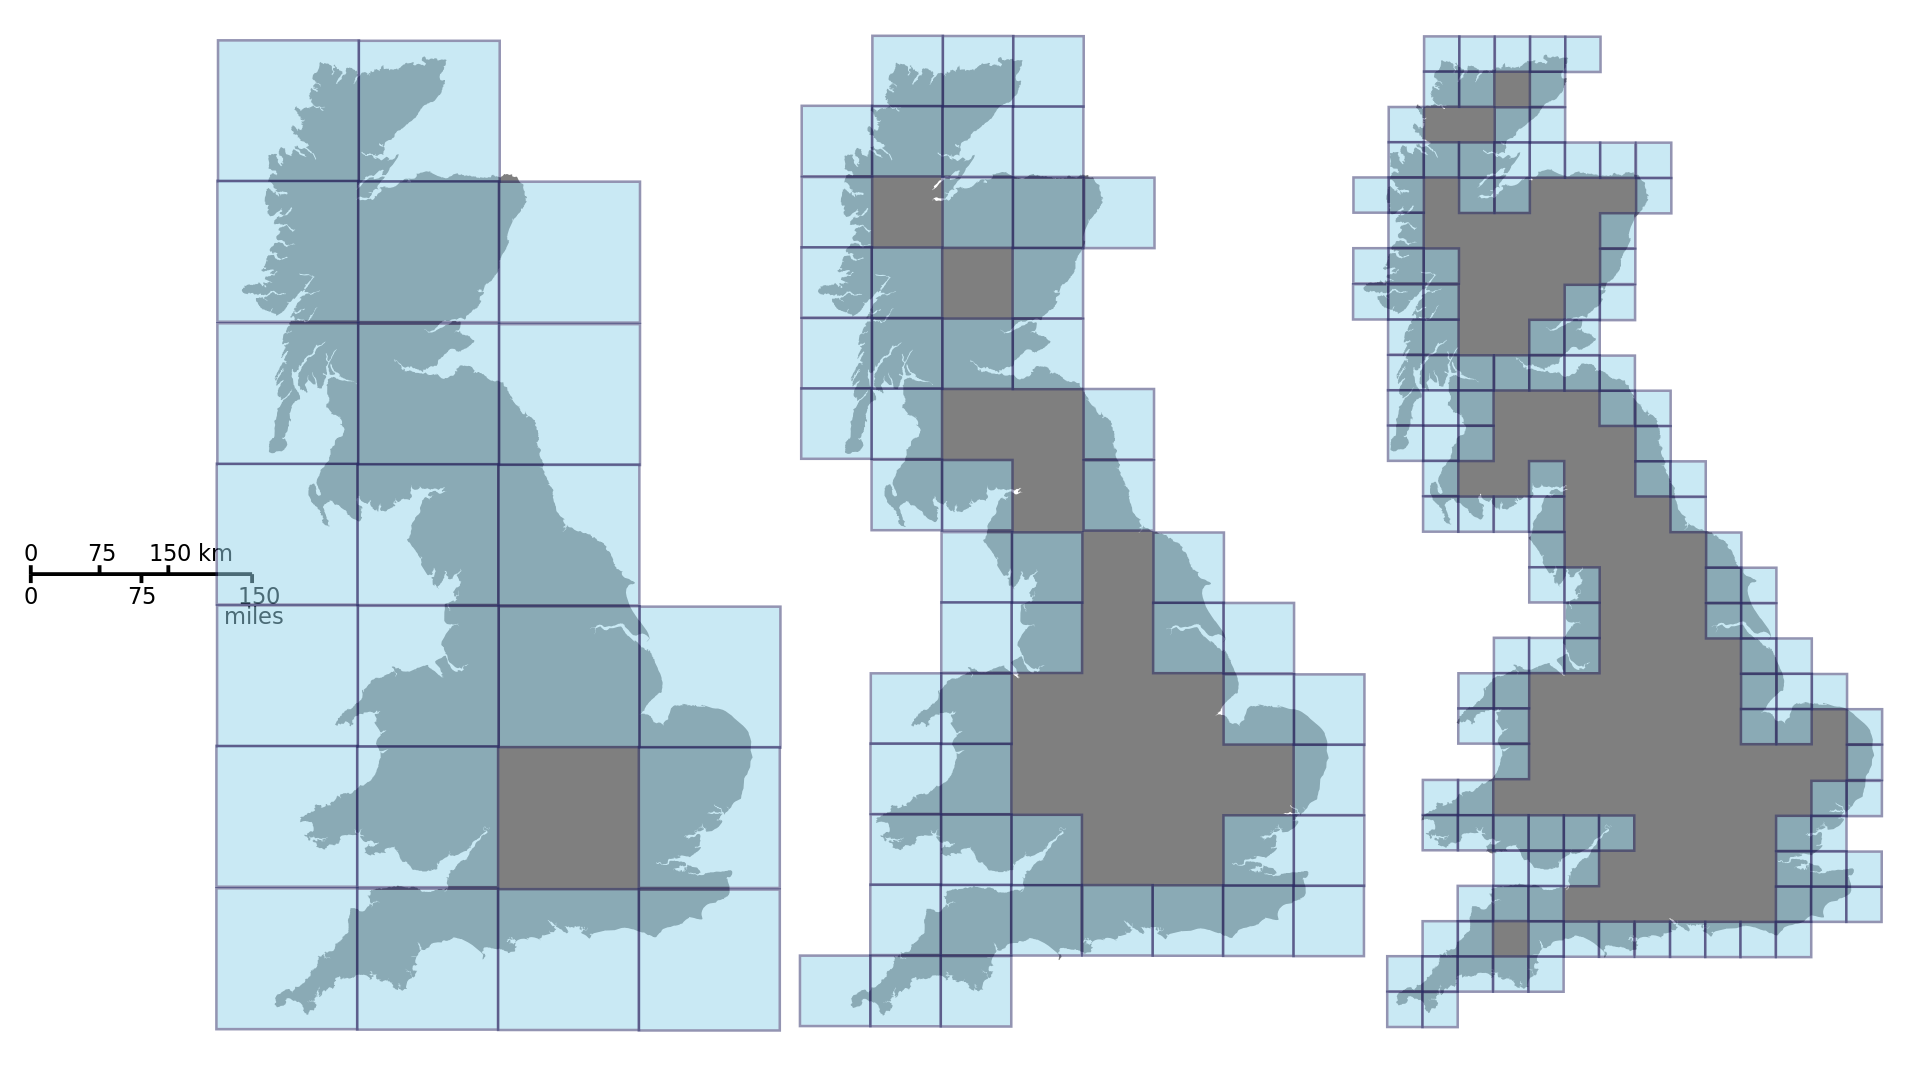
\includegraphics[width=\textwidth]{GB_box.png}
        \caption{An example of box coverings of the coast line of Great Britain.  Created by Alexis Monnerot-Dumaine (CC BY-SA 3.0)}
        \label{fig:box_covering}
    \end{figure}

    While both of these methodologies are commonly used, neither is the only one available for either task.  Of particular interest is a related threshold based method for the extraction of river networks where the threshold is a combination of support area and slope.  \textbf{Both the methodology and the threshold chosen will significantly impact the extracted channel network.}
  \end{block}


\end{column}

\separatorcolumn

\begin{column}{\colwidth}

  \begin{alertblock}{Significant differences in fractal parameters from area and slope-area based channel extractions}

    For a landscape generated with a simple stream power model \cite{braun2013very} river networks were extracted across a range of thresholds of both support area as well as slope and support area.  \textbf{Different values of fractal dimension, and styles of response were found across the the two methodologies}.  Channel extraction parameters must be justified before a meaningful fractal analysis can be conducted.

  \end{alertblock}

  \begin{block}{Changes in fractal parameters due to channel extraction choices}
  When looking at fractal dimension calculated with a simple support area threshold (figure \ref{fig:area_fractal}), akin to Tarboton et al. \cite{tarboton1988fractal}, we see a very similar response to their results, with a fractal dimension close to 1 at smaller scales, and a fractal dimension close to 2 at larger scales.  However, when using a slope and area threshold, we see results that are much closer to one fractal dimension across all scales (figure \ref{fig:slopearea_fractal}).  For consistency both datasets were fit by a piecewise function with 2 linear components.  This is clearly necessary to fit the data in figure \ref{fig:area_fractal}, but not so for figure \ref{fig:slopearea_fractal}.
  \begin{figure}[ht]
  %\begin{subcaptiongroup}
  \begin{subfigure}{.45\textwidth}
      \centering
      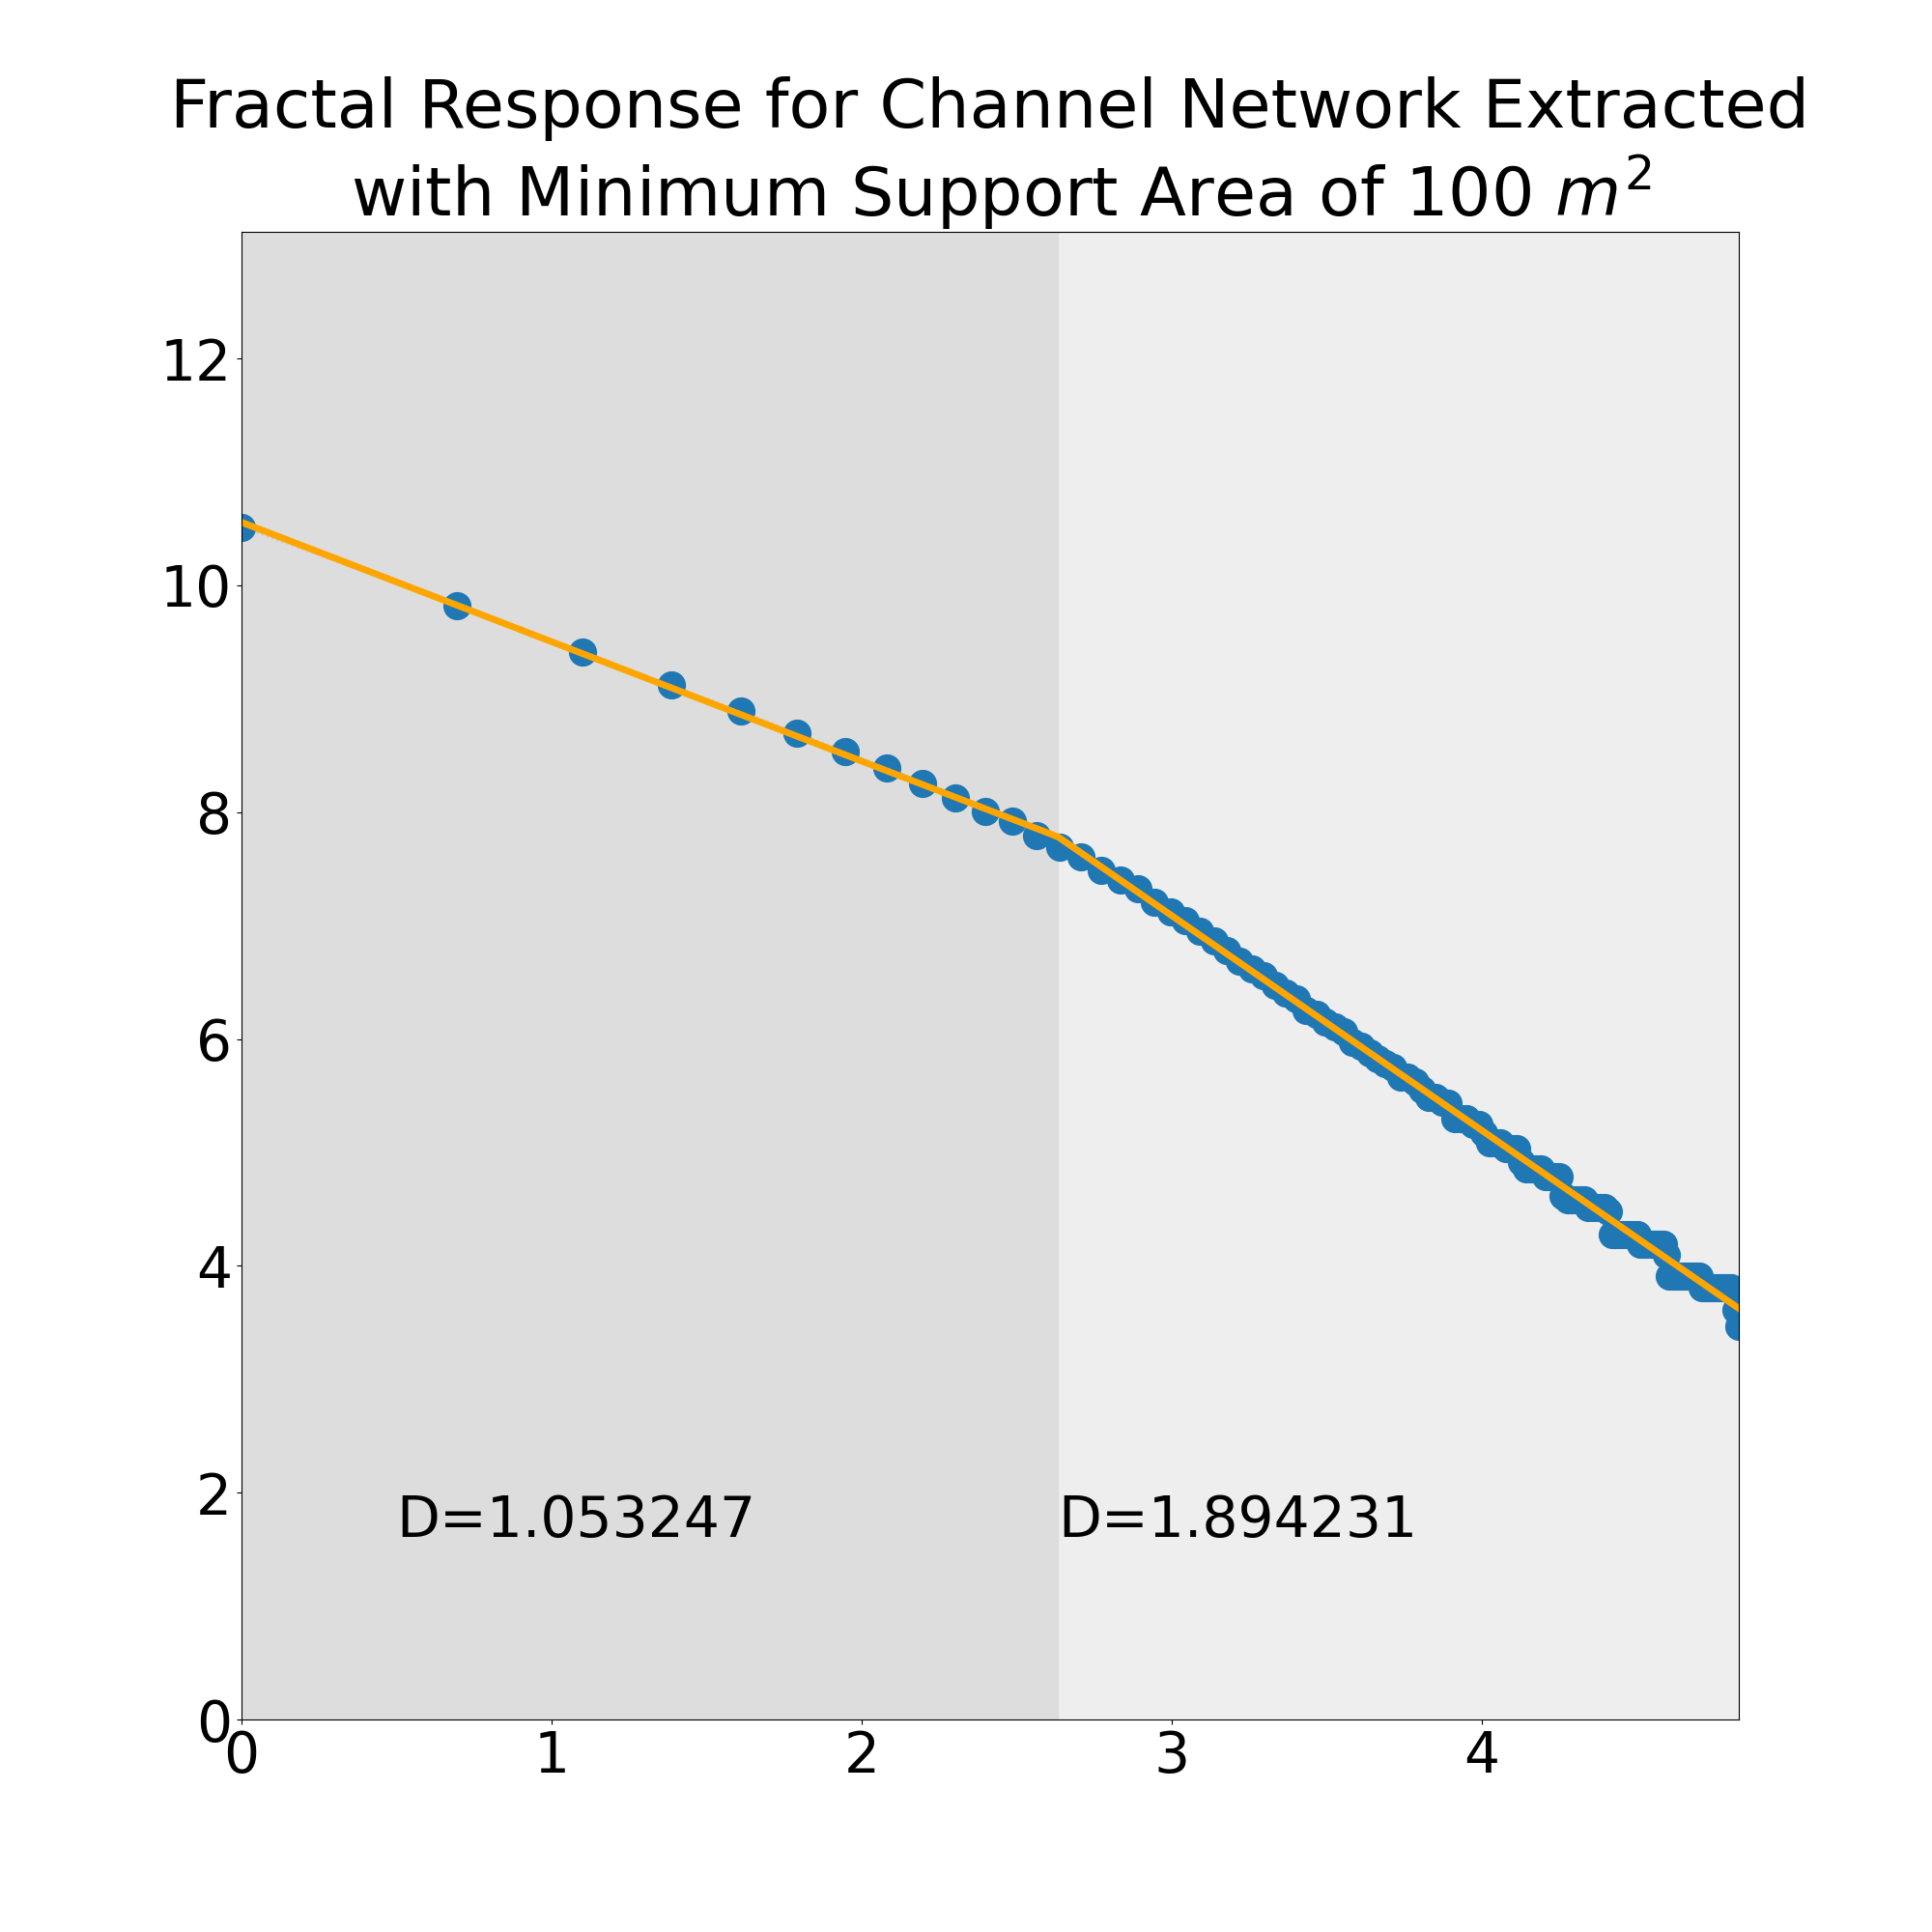
\includegraphics[width=\textwidth]{area_fractal.png}
      \caption{Support area only.}
      \label{fig:area_fractal}
  \end{subfigure}
  \begin{subfigure}{.45\textwidth}
      \centering
      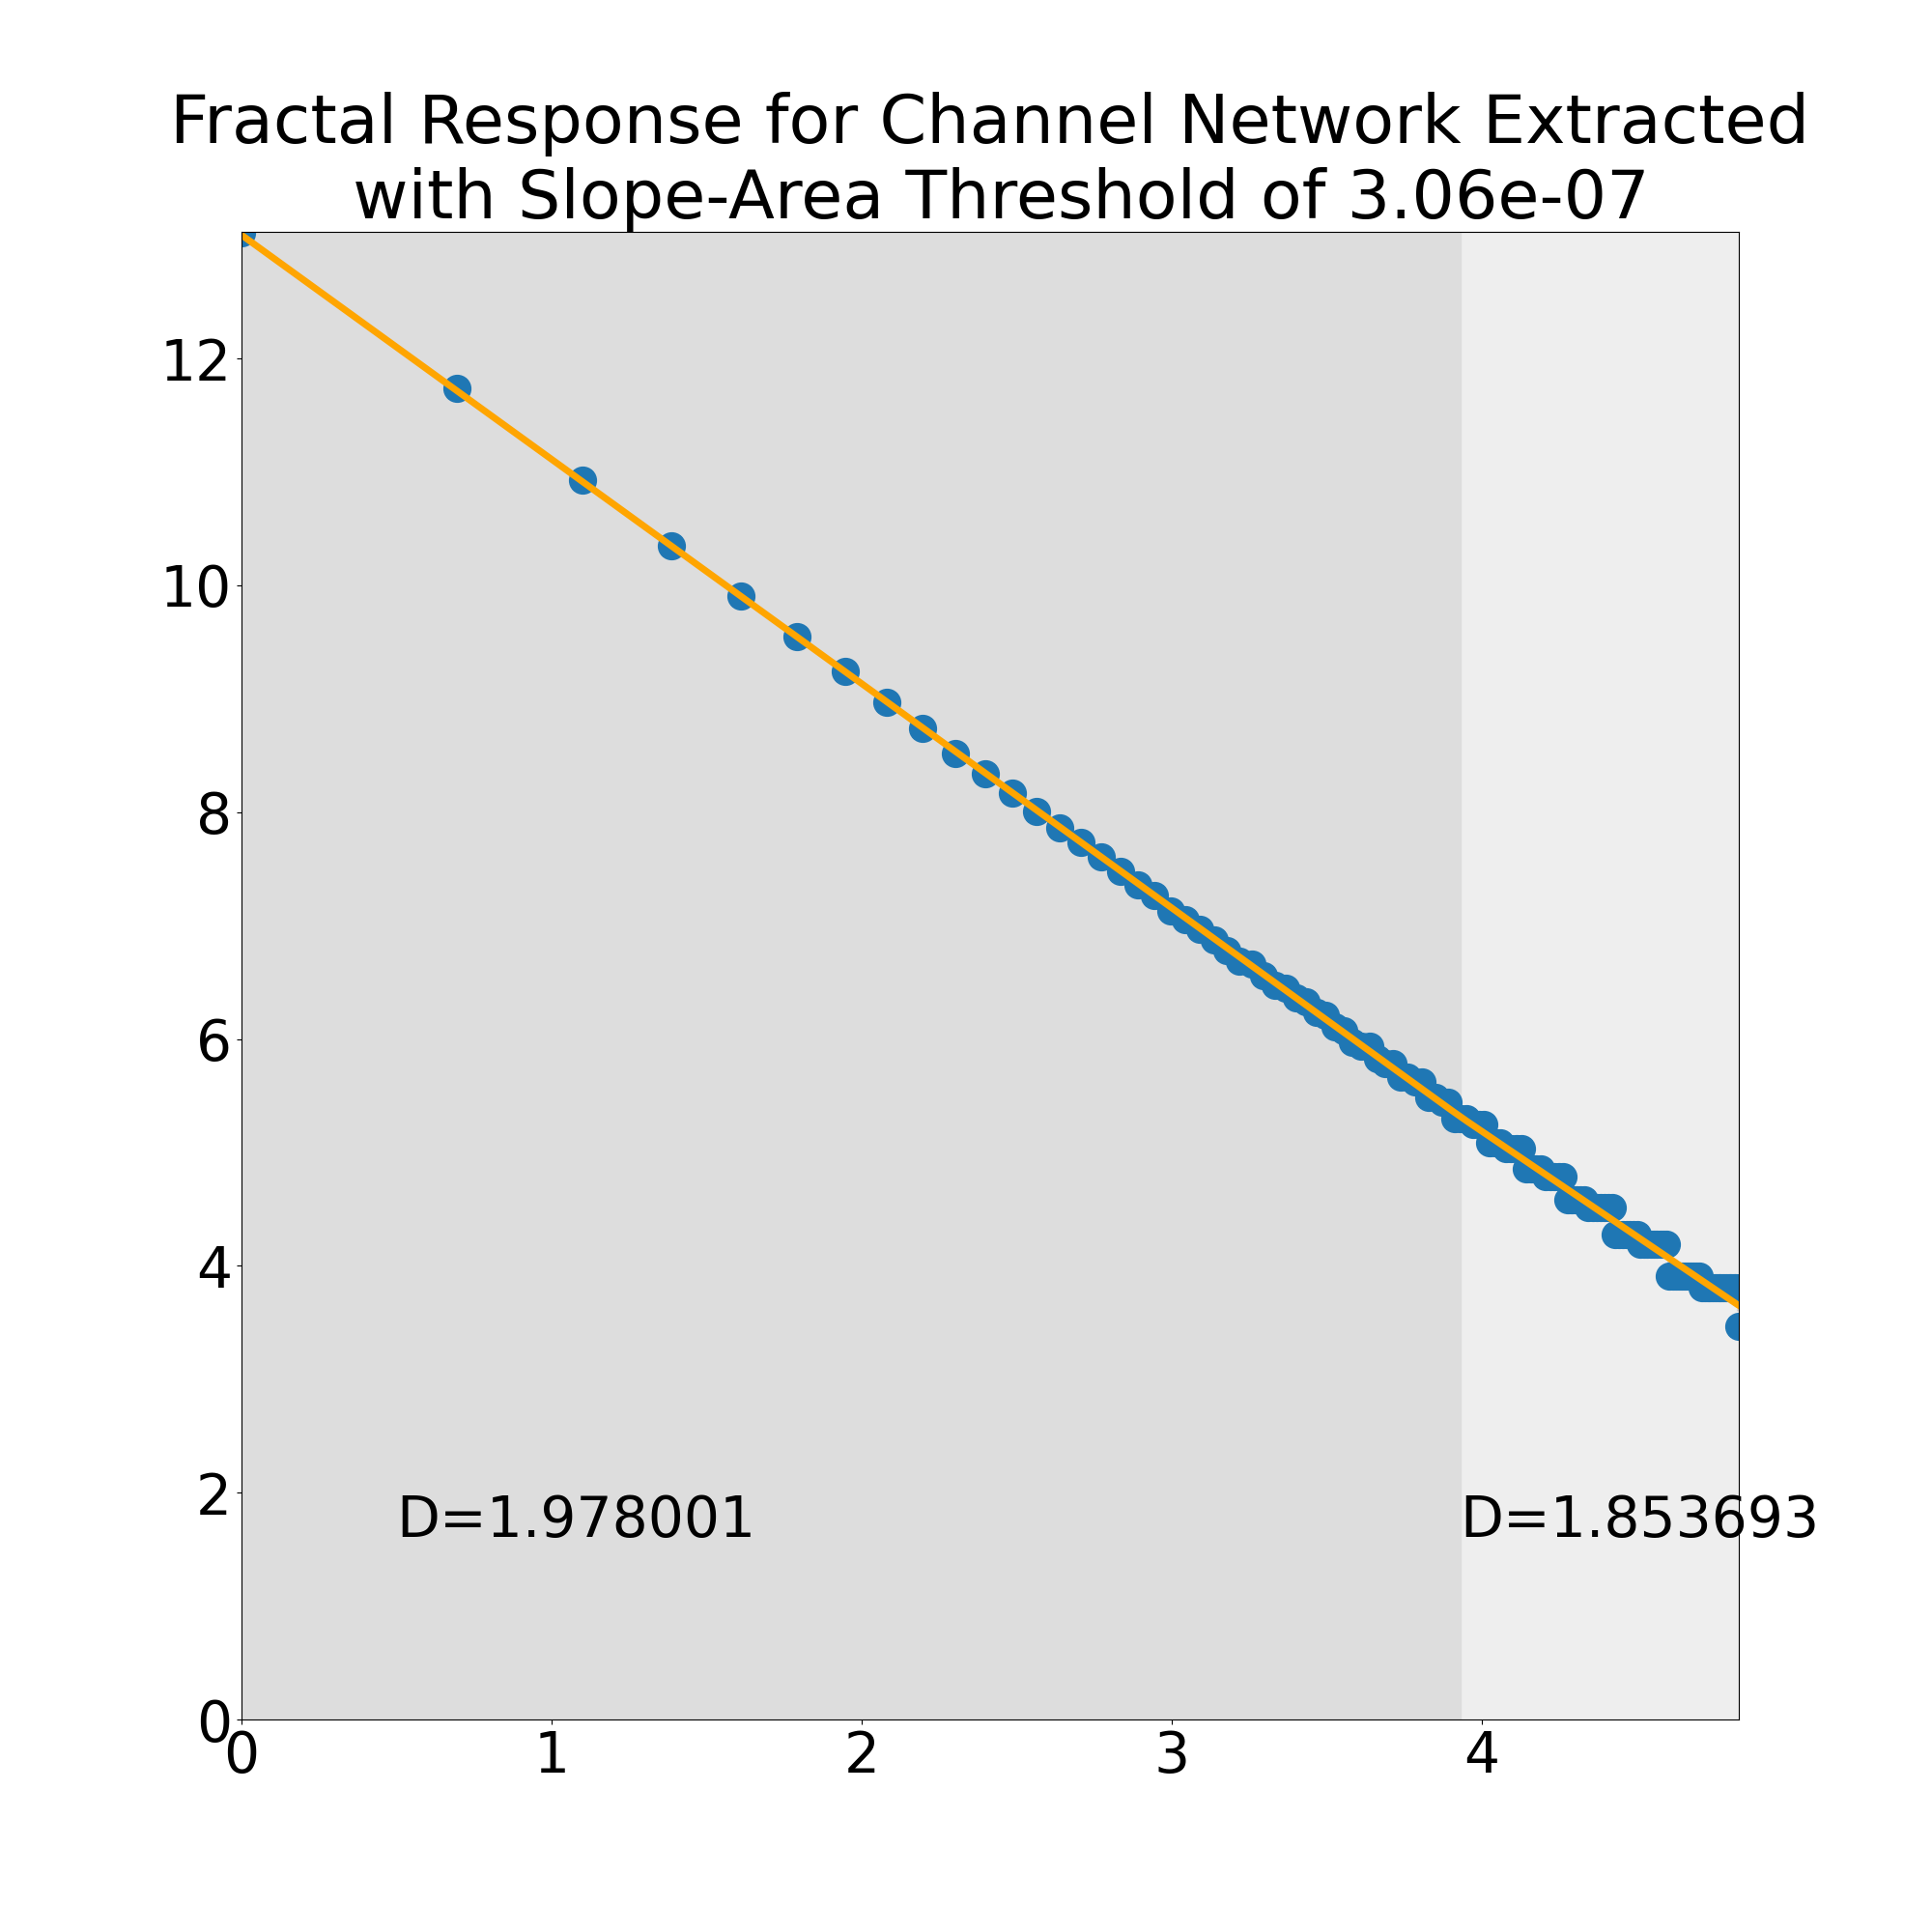
\includegraphics[width=\textwidth]{slopearea_fractal.png}
      \caption{Slope and support area.}
      \label{fig:slopearea_fractal}
  \end{subfigure}
 % \end{subcaptiongroup}
 \caption{Fractal response for two different channel extraction methods.}
    \end{figure}
  \end{block}

  Not only do we see vastly different responses between the two methodologies, we see that extracted fractal parameters display systematic dependence on the thresholds chosen for channel extraction (figure \ref{fig:transition_area}, \ref{fig:dim_area}).

  \begin{figure}
  \begin{subfigure}{.45\textwidth}
       \centering
      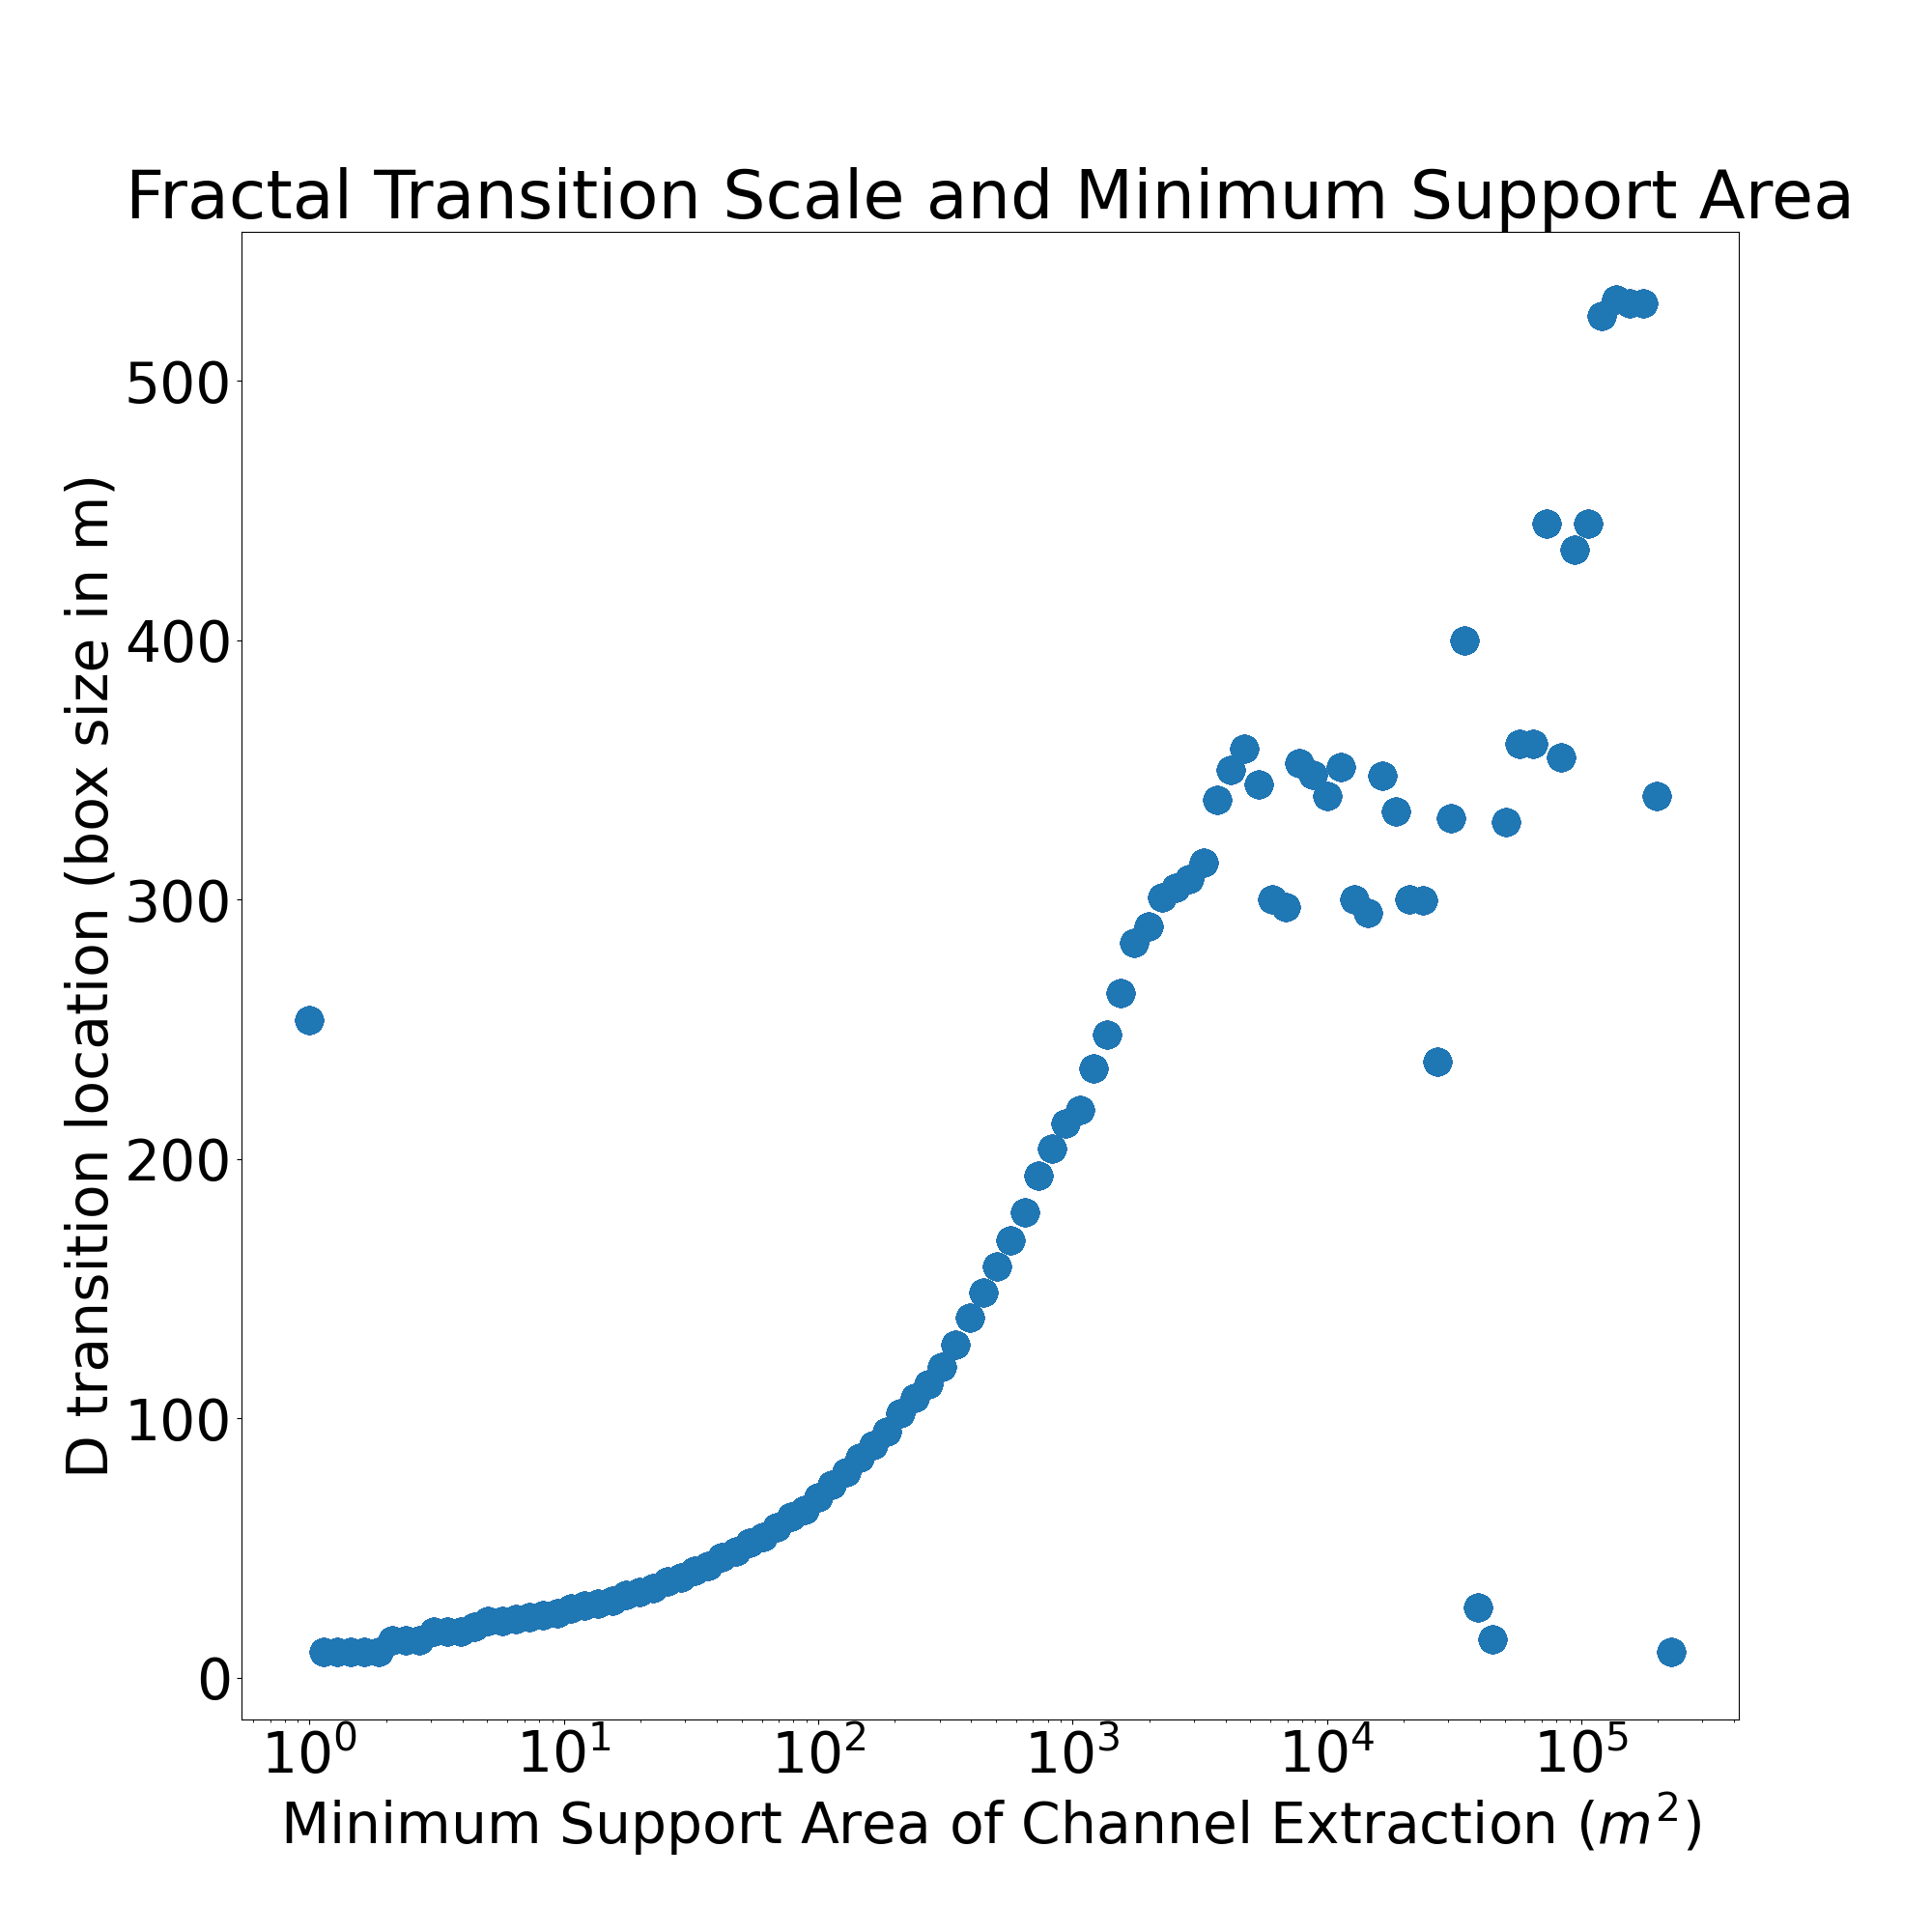
\includegraphics[width=\textwidth]{transition_and_area.png}
      \caption{Location of the transition between fractal dimensions.}% as a function of minimum support area.}
      \label{fig:transition_area}
    \end{subfigure}
    \begin{subfigure}{.45\textwidth}
            \centering
      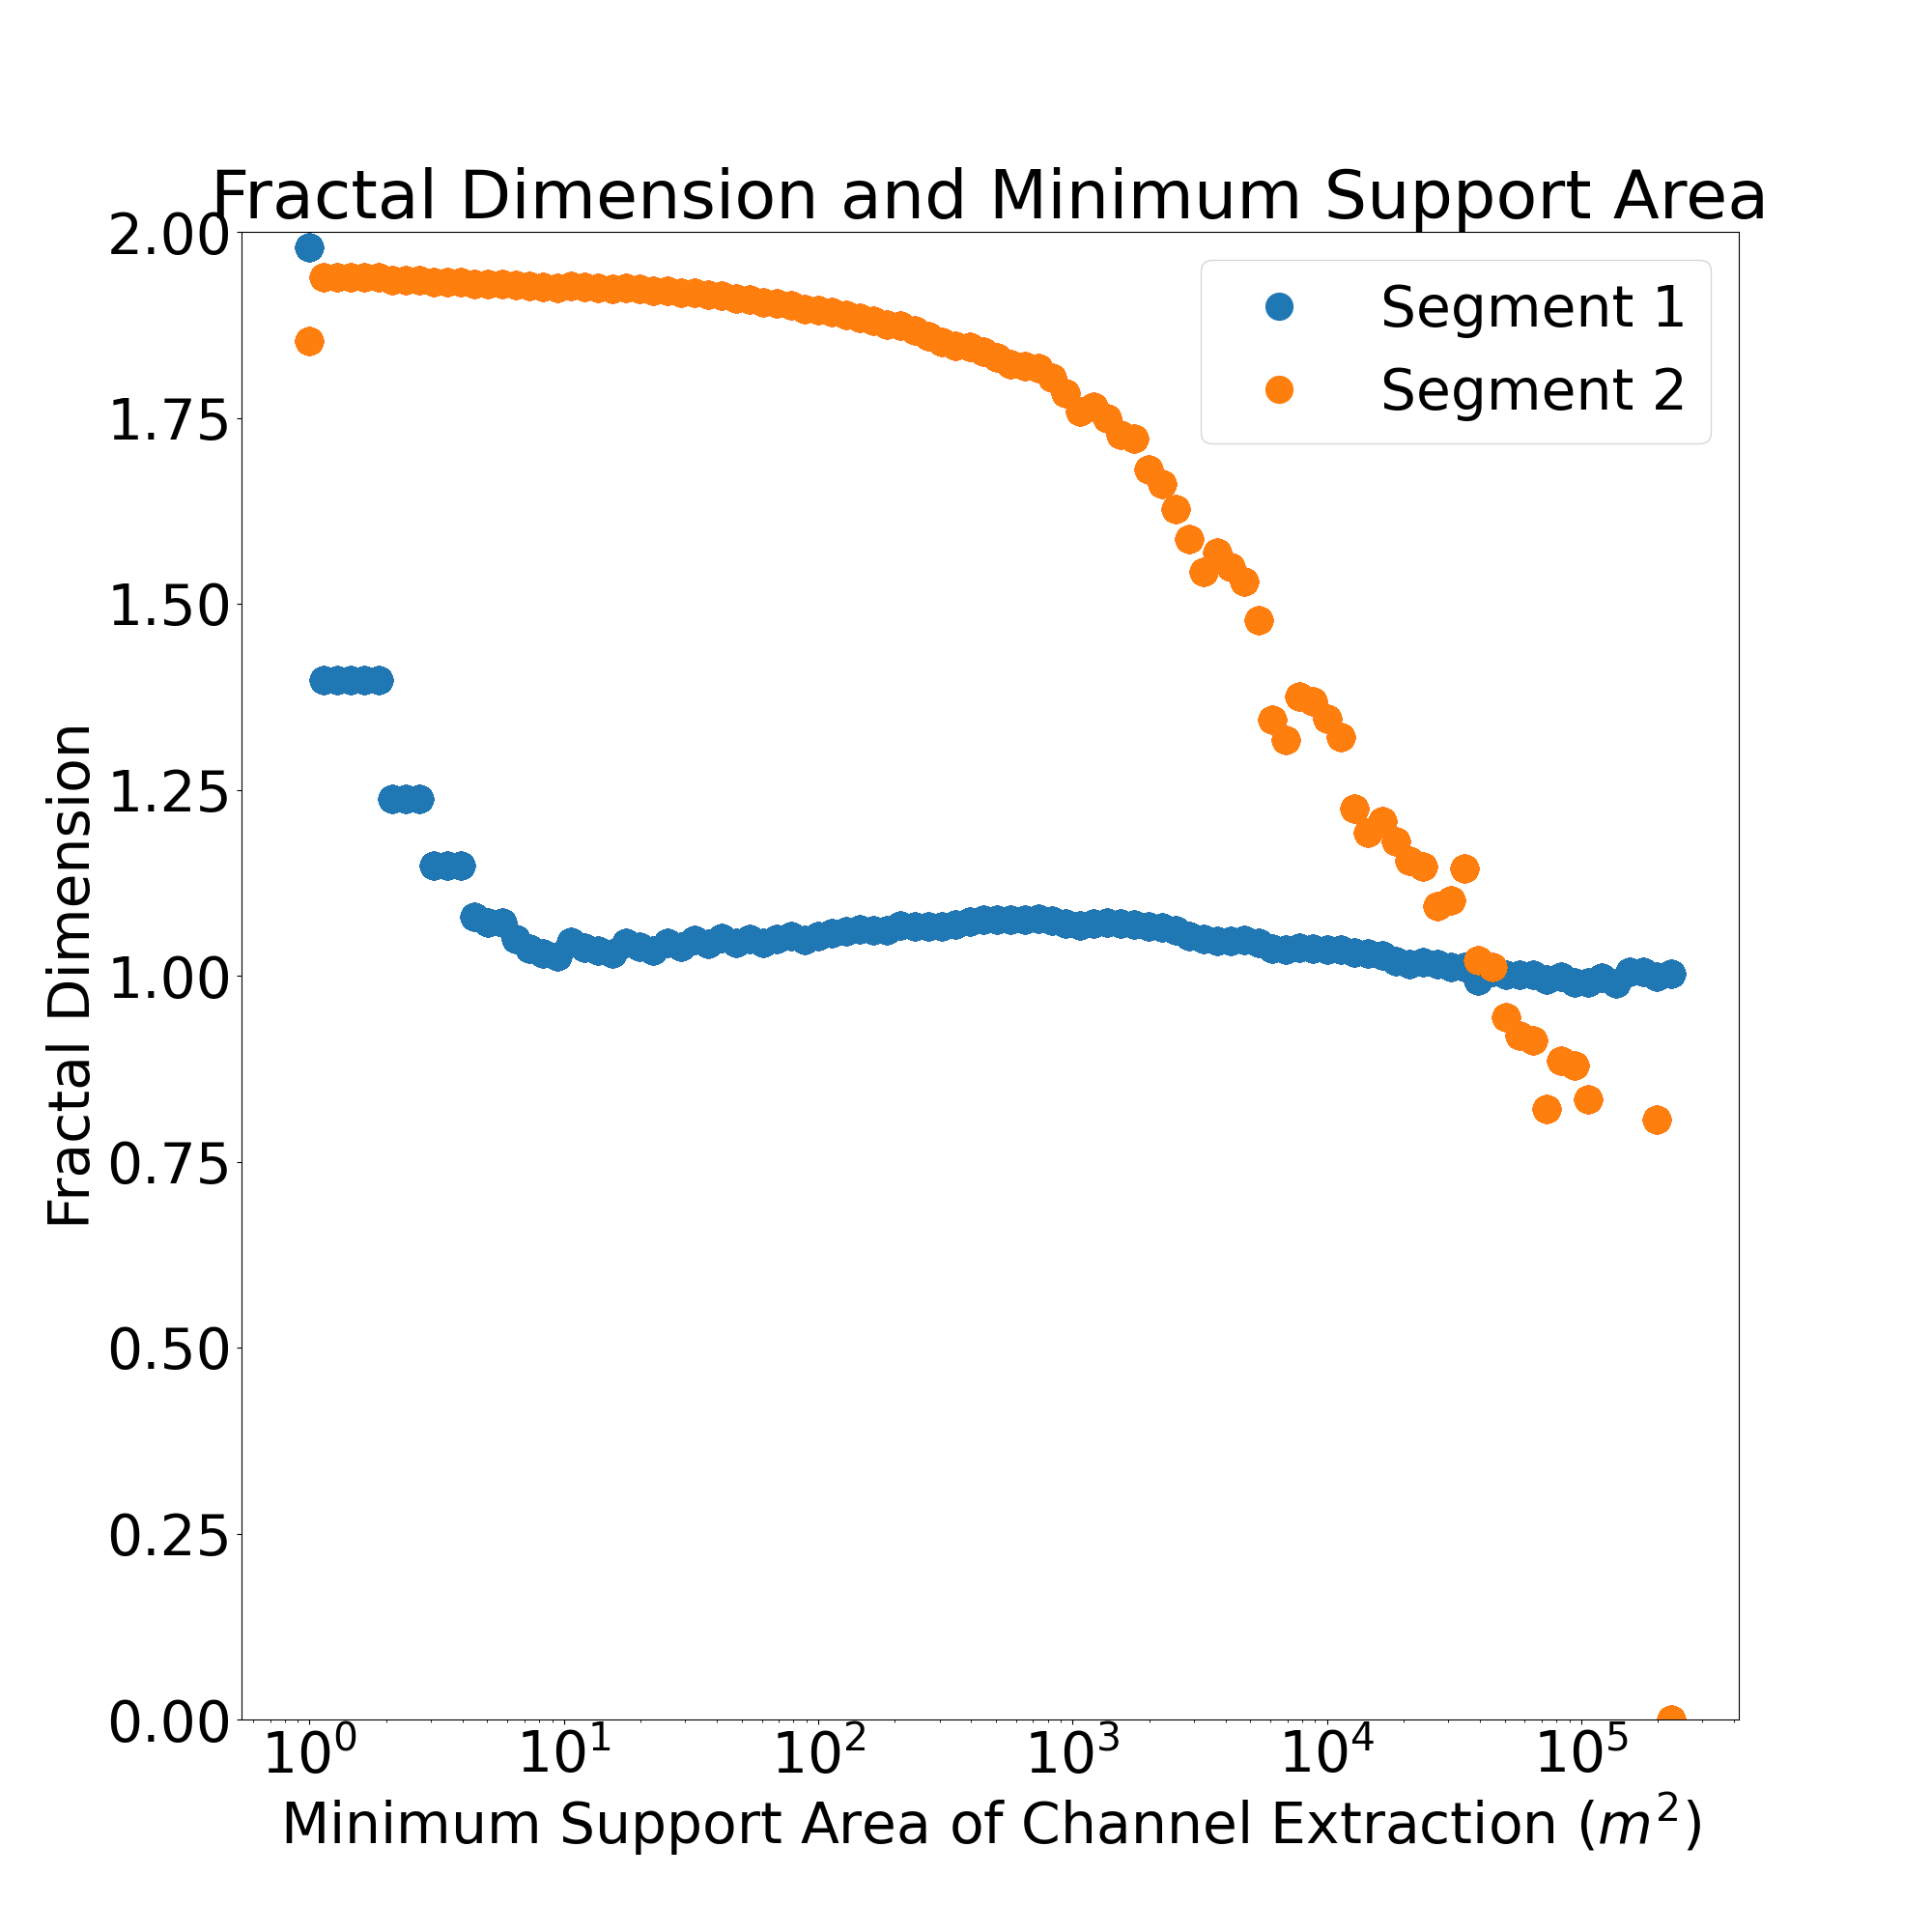
\includegraphics[width=\textwidth]{D_and_area.png}
      \caption{Fractal dimension as a function of minimum support area.}
      \label{fig:dim_area}
    \end{subfigure}
    \caption{Parameters of the fractal dimension show systematic dependency on the minimum support area used for channel extraction.}
  \end{figure}

 

\end{column}

\separatorcolumn

\begin{column}{\colwidth}

  \begin{block}{Are classic fractal results a product of network extraction choices?}

    \begin{figure}
        \centering
        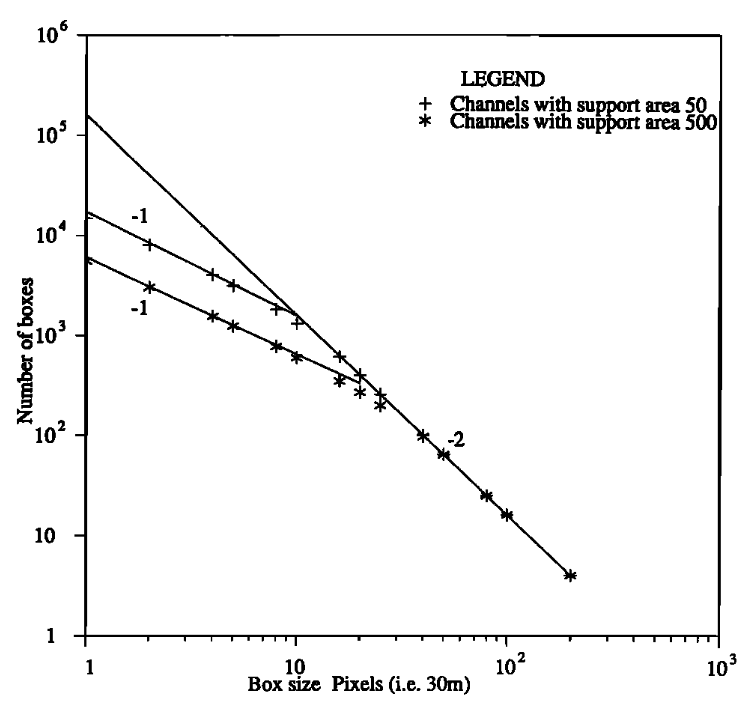
\includegraphics[width=0.5\textwidth]{tarboton.png}
        \caption{Box Counting Results from Tarboton et al. \cite{tarboton1988fractal}}
        \label{fig:tarboton}
    \end{figure}
   My results on the box counting based fractal dimension for channel networks extracted with a minimum support area threshold are very similar to those found by Tarboton et al. who also used a minimum support area threshold \cite{tarboton1988fractal}.  They interpreted their results in the lens of Mandelbrot's Peano curve based model of river networks.  Mandelbrot constructed a curve where individual segments had dimension slightly above 1, which was supposed to represent sinuousity, whereas the network as a whole had a fractal dimension close to 2, which represented the space filling nature of the river network \cite{mandelbrot1982fractal}.  Tarboton et al. interpreted their results to uphold Mandelbrot's model.  However, it may be that this was simply an artifact of using a support area only based extraction method.
  \end{block}

\begin{alertblock}{Conclusions and next steps}
    \begin{itemize}
        \item Fractal Results are very dependent on decisions made at the channel extraction step.
        \item Channel extraction decisions must be well justified prior to the interpretations of fractal results.
        \item The analysis should be re-done with a slope-area function justified from the literature.
        \item The analysis should be re-done on a real landscape.
        \item More work is needed to understand how and why these decisions influence the results in the way they do.
        \item More work is needed to understand the influence of different methodologies used to calculate the fractal dimension.
    \end{itemize}
\end{alertblock}

  \begin{block}{References}

    \nocite{*}
    \footnotesize{\bibliographystyle{plain}\bibliography{poster}}

  \end{block}

\end{column}

\separatorcolumn
\end{columns}
\end{frame}

\end{document}
